% Chapter 3

\chapter{Deep neural networks for identification} % Main chapter title

\label{Chapter3} % For referencing the chapter elsewhere, use \ref{Chapter1} 

\lhead{Chapter 3. \emph{Deep neural networks for identification}} % This is for the header on each page - perhaps a shortened title

%----------------------------------------------------------------------------------------



\section{Sequence neural networks}

Recurrent neural networks (RNN), long short-term memory (LSTM) \cite{hochreiter1997long} and gated recurrent neural networks (GRU) \cite{chung2014empirical} can model complex sequences and have been used for sequence modeling problems.

Our deep learning model is implemented as an attentional encoder network (Figure \ref{fig:encoder}). An input sequence  $\mathbf{x = (x_{1} , \ldots{} , x_{m} )}$  and calculates a forward sequence of hidden states  ($\mathbf{\overrightarrow{h_{1}}}$,\ldots{},$\mathbf{ \overrightarrow{h_{m}}}$). The hidden states $\mathbf{\overrightarrow{h_{j}}}$  are averaged to obtain the attention vector $\mathbf{h_{j}}$ representing the context vector from the input sequence.

Embedding layer maps discrete input words to dense vectors for computational efficiency before feeding this sequence to LSTM/GRU Layers. The attentional network could learn how to extract suitable features from the raw data and can attend to previous DNA nucleotide within the same input sequence. 

LSTM encoder have 3 gates to protect and control the cell state, the input gate denoted $\mathbf{i}$ which defines how much of the newly computed state you want to let through, forget gate denoted $\mathbf{f}$ that decides what information is to be kept and what is to be thrown away,  the output of the update gate denoted $\mathbf{U}$ that's used to update the cell state and the output of the LSTM cell $\mathbf{o}$ .$\mathbf{W}$ is the recurrent connection at the previous hidden layer and current hidden layer and $\mathbf{C}$ is the internal memory of the unit  as shown in the following equations \newline
$\mathbf{i_{t}=\sigma(x_{t}U^i + h_{t-1}W^i)}$ \newline
$\mathbf{f_{t}=\sigma(x_{t}U^f + h_{t-1}W^f)}$ \newline
$\mathbf{o_{t}=\sigma(x_{t}U^o + h_{t-1}W^o)}$. 

GRU encoder is same as LSTM except it has only 2 gates, Reset gate denoted $\mathbf{r}$ that determines how to combine the new input with the previously saved input state and the update gate denoted $\mathbf{z}$ that defines the amount of information to keep around, as defined  in the following equations \newline
$\mathbf{z_{t}=\sigma(x_{t}U^z + h_{t-1}W^z)}$ \newline
$\mathbf{r_{t}=\sigma(x_{t}U^r + h_{t-1}W^r)}$ \newline
$\mathbf{\overline{h_{t}} = tanh(x_{t}U^h + (r_{t} * h_{t-1})W^h )}$ \newline
$\mathbf{ h_{t} = (1-z_{t})h_{t-1} +z_{t}\overline{h_{t}}}$.


The attentional neural model was trained with the DNA nucleotide bases with fragments with different lengths. The model will predict in a binary output format whether this fragment is viral or non-viral.

The top-performing model (Figure \ref{fig:model_diagram}) consists of an input embedding layer of size 128 mapping input DNA nucleotide tokens into an embedding space, that is fed to an LSTM layer. The forward sequence $\mathbf{\overrightarrow{h_{j}}}$ is then averaged together to create an attentional vector representing token context within the same fragment. A dropout layer was added after the attentional layer to avoid overfitting over the input data.

LSTM layer was performing better as in \ref{table:hyper_results} than the GRU cell. GRU encoder having less gates than LSTM model make it faster and easier to converge, but depedending on the size and the format of the input data. LSTM with more gates would be slower but will outperform GRU encoder type.

The input sequence is divided into 5 grams sized tokens these tokens are then treated as a single word (Figure \ref{fig:encoder}). This single token is mapped as a point in the embedding space created during training the neural model.

During training, all parameters are optimized jointly using Adam to maximize the conditional probability of tokens found together to predict if an input sequence is viral or not.

In this model, an early stopping mechanism was used as a form of regularization to avoid over-fitting over the data while making more epochs over the data. The early stopping mechanism was used with patience of 3 non -improving consecutive epochs; the neural model will stop training while saving the latest improving checkpoint over the validation set defined.

\subsection{Attention mechanism}


\LaTeX{} is not a WYSIWYG (What You See is What You Get) program, unlike word processors such as Microsoft Word or Apple's Pages. Instead, a document written for \LaTeX{} is actually a simple, plain text file that contains \emph{no formatting}. You tell \LaTeX{} how you want the formatting in the finished document by writing in simple commands amongst the text, for example, if I want to use \textit{italic text for emphasis}, I write the `$\backslash$\texttt{textit}\{\}' command and put the text I want in italics in between the curly braces. This means that \LaTeX{} is a ``mark-up'' language, very much like HTML.

\section{Convolution neural networks}

\LaTeX{} is not a WYSIWYG (What You See is What You Get) program, unlike word processors such as Microsoft Word or Apple's Pages. Instead, a document written for \LaTeX{} is actually a simple, plain text file that contains \emph{no formatting}. You tell \LaTeX{} how you want the formatting in the finished document by writing in simple commands amongst the text, for example, if I want to use \textit{italic text for emphasis}, I write the `$\backslash$\texttt{textit}\{\}' command and put the text I want in italics in between the curly braces. This means that \LaTeX{} is a ``mark-up'' language, very much like HTML.

\subsection{Triplet loss mechanism}


\LaTeX{} is not a WYSIWYG (What You See is What You Get) program, unlike word processors such as Microsoft Word or Apple's Pages. Instead, a document written for \LaTeX{} is actually a simple, plain text file that contains \emph{no formatting}. You tell \LaTeX{} how you want the formatting in the finished document by writing in simple commands amongst the text, for example, if I want to use \textit{italic text for emphasis}, I write the `$\backslash$\texttt{textit}\{\}' command and put the text I want in italics in between the curly braces. This means that \LaTeX{} is a ``mark-up'' language, very much like HTML.

%----------------------------------------------------------------------------------------



\subsection{Hyperparameters optimization}

Model parameters affect the performance of the deep learning model, and they control the behavior of the training algorithm as well. We selected the grid search technique in order to find the most suitable parameters. The grid search is considered a traditional technique for hyperparameters optimization and it brute force different combinations. We ran several experiments on 20\% of our training set for 500 bp. Then, we divided it into training, validation, and testing set with the following percentages 70\%, 10\%, and 20\%. These experiments were designed to find the best parameters for the number of recurrent layers, the embedding size for each layer and the input sub-words (ngram). Our reported results (Table \ref{table:hyper_results}) show that the best parameters setup is for 2 layers, 128 embedding size, and 5 ngram. 

We ran other experiments with the same parameters to check the ability of our model with other configuration, so we changed different parameters separately such as embedding size to 256 neurons, the number of layers to 3 and the recurrent cell type to GRU instead of LSTM. We found a slightly less accuracy and ROC-AUC scores but the training time was much more than the best parameters configuration as expected due to increasing number of neural network parameters.

\begin{table}[!htbp]
	\centering
	\begin{tabular}{||c c c c c||} 
		\#Layers & Embedding & Ngram & ROC-AUC & Accuracy \\ [0.5ex] 
		\hline\hline
		1      & 32                      & 3     & 0.8     & 73.66    \\
		1      & 32                      & 5     & 0.83    & 76.42    \\
		1      & 32                      & 7     & 0.79    & 72.11    \\
		1      & 64                      & 3     & 0.83    & 76.1     \\
		1      & 64                      & 5     & 0.83    & 75.98    \\
		1      & 64                      & 7     & 0.77    & 69.96    \\
		1      & 128                     & 3     & 0.83    & 75.76    \\
		1      & 128                     & 5     & 0.85    & 77.41    \\
		1      & 128                     & 7     & 0.78    & 70.93    \\
		2      & 32                      & 3     & 0.8     & 73.25    \\
		2      & 32                      & 5     & 0.83    & 76.49    \\
		2      & 32                      & 7     & 0.79    & 72.82    \\
		2      & 64                      & 3     & 0.81    & 73.96    \\
		2      & 64                      & 5     & 0.84    & 76.46    \\
		2      & 64                      & 7     & 0.78    & 72.53    \\
		2      & 128                     & 3     & 0.83    & 76.15    \\
		\textbf{2} & \textbf{128}            & \textbf{5} & \textbf{0.85} & \textbf{77.9} \\
		2      & 128                     & 7     & 0.78    & 70.63    \\[1ex]
	\end{tabular}
	\caption{Hyperparamters optimization results}
	\label{table:hyper_results}
\end{table}


\begin{figure}[!htbp]
	\centering
	\begin{subfigure}{0.5\textwidth}
		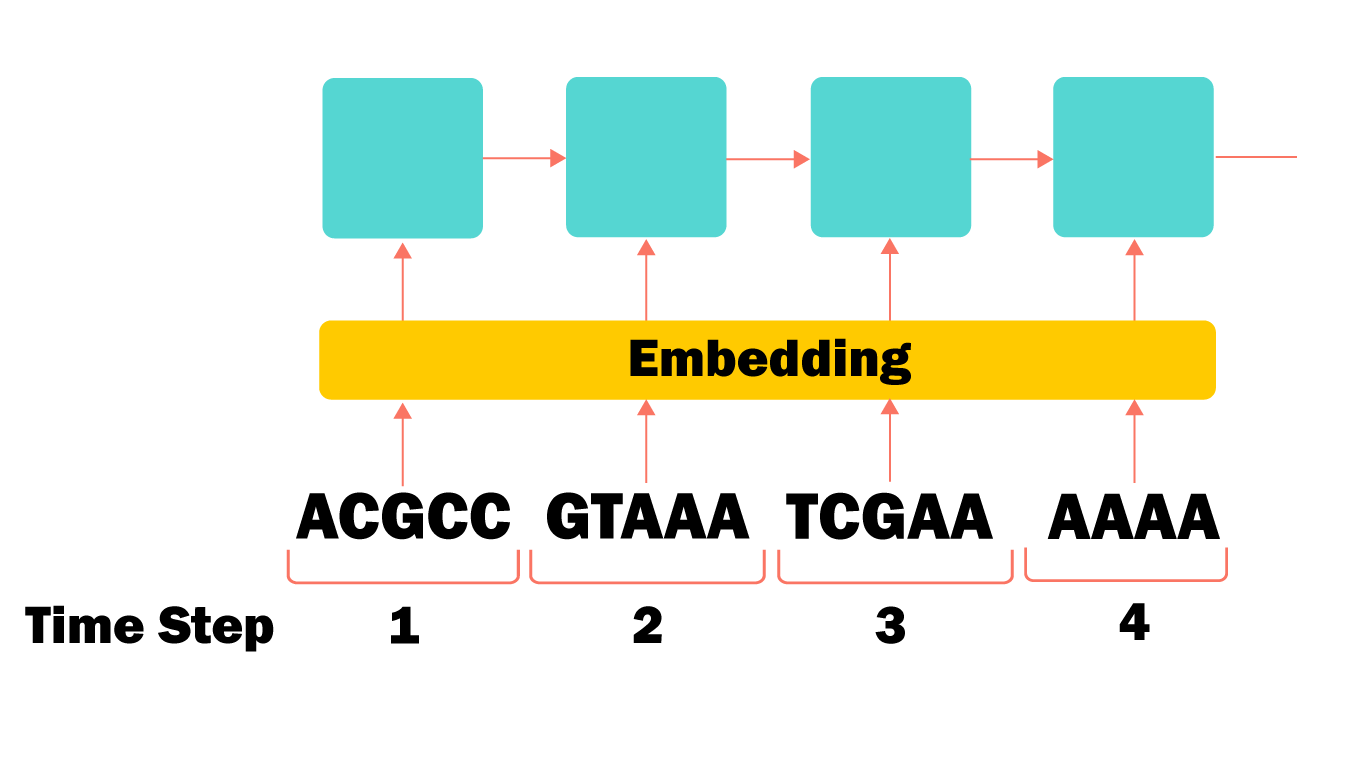
\includegraphics[width=\linewidth]{Pictures/encoder.PNG}
		\caption{Embedding Layer} 
		\label{fig:encoder}
	\end{subfigure}
	\hspace*{\fill} % separation between the subfigures
	\begin{subfigure}{0.5\textwidth}
		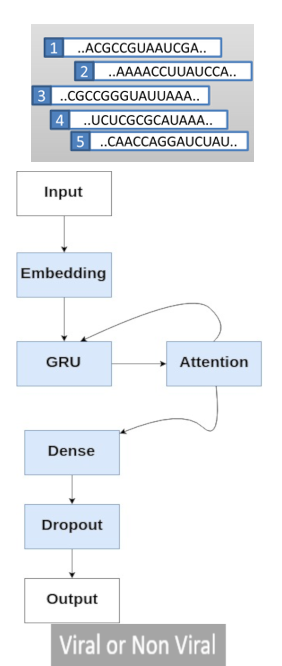
\includegraphics[width=\linewidth]{Pictures/model_diagram.PNG}
		\caption{Neural network model architecture} 
		\label{fig:model_diagram}
	\end{subfigure}
	\caption{VirNet model} 
	\label{fig:model_arch}
\end{figure}

